\chapter{Resultados Esperados}
\label{chap:ResultadosEsperados}

O algoritmo de visão computacional será implementado e avaliado sua acurácia para detectar obstáculos em tempo real, durante a movimentação do RMA. A aplicação visa desviar destes obstáculos, imitando um campo minado. O algoritmo de controle desempenhará o papel de planejar as novas trajetórias para a movimentação.

O RMA será prototipado utilizando um Raspberry Pi e um Arduino, onde serão integrados os sensores e atuadores. Este contará com um chassi visto na Figura~\ref{fig:chassi}, motores, rodas, sensores de imagem e ultrassônicos. A programação será realizada em C para o Arduino, pela Arduino IDE, onde será definido sua lógica de movimentação; e em Python para o Raspberry Pi que irá tratar a detecção dos objetos.

Os sensores ultrassônicos atuarão como última ação do RMA, caso o sistema de visão computacional ou o controle de sua trajetória falhe.

\begin{figure}[!hbtp]
  \centering
   \caption{Chassi.}
    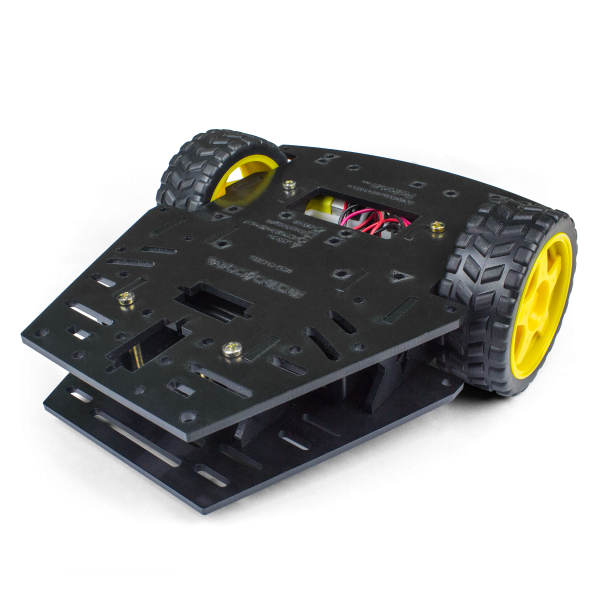
\includegraphics[width = 0.8\textwidth]{Caps/Figs/resultados/582_1_H.png}
   \label{fig:chassi}
    \fonte{Robocore}
\end{figure}
